% =====================================================================
% Part 2: Polyfit detector, controllers, metrics, results, conclusion
% (sections 7-11). Included by explanation.tex.
% =====================================================================

\section{Detector 3 -- Polynomial Fit in Bird's-Eye View}
\label{sec:polyfit}

We now arrive at the proposed detector. It is the most involved
pipeline in this report, but every stage is motivated by a concrete
failure mode of the Hough baseline. Before plunging into homographies
and sliding windows, let us reconstruct why a different model class is
needed at all.

\subsection{Motivation: why straight lines are the wrong model}

In Section~\ref{sec:hough} of Part~1 we saw that the Hough detector
collapses each lane boundary down to a single straight segment. On a
tight bend this is a structurally biased estimator: the line of best
fit through a curved set of edge pixels lies somewhere inside the
curve, so the implied lane centre drifts toward the inside of the
turn, and the predicted heading is off by the angular gap between the
chord and the tangent. The faster the curve, the worse the gap.

A natural fix is to let the model class be curved. The simplest curved
model is a parabola, $x = a y^2 + b y + c$, which has exactly enough
freedom to capture the principal bend of a road segment without
overfitting to noise. Once we commit to a curved model, however, two
problems appear.

\begin{intuition}
Think about what equally-spaced lane markings look like in the
forward-perspective image: the dashes near the car span dozens of
pixels each, while the dashes far ahead occupy only a couple of
pixels. A polynomial fit weighted by pixel count is therefore
dominated by what is close, and the far-field information that matters
for anticipating curves is essentially thrown away. To use a curved
model honestly, we first have to undo the perspective distortion.
\end{intuition}

The second problem is that even with a curved model, fitting it on the
raw image still has to deal with foreshortening: a constant lane width
in world coordinates corresponds to a width in image coordinates that
shrinks like $1/v$ as you go up the image. The natural solution to
both problems is the same: warp the image to a top-down bird's-eye
view (BEV) first, fit the polynomial in that metric-friendly frame,
and project the result back when we need to draw on the camera image.
This is the central idea of \texttt{lane\_methods.py:PolyFitDetector}.

\subsection{The lane-pixel mask}

The pipeline begins with a binary mask flagging every pixel that
``looks like a lane marking''. The detector composes three orthogonal
sources of evidence
(\texttt{lane\_methods.py:PolyFitDetector.\_lane\_pixels}):
\begin{enumerate}[leftmargin=1.8em,itemsep=2pt]
  \item A horizontal Sobel response, normalised by its per-frame
        maximum, thresholded at $60/255$.
  \item An HSV white mask: $S<70$ and $V>170$.
  \item An HSV yellow mask: $15<H<40$, $S>60$, $V>130$.
\end{enumerate}
The combined mask is the bitwise OR of these three. Written as a
predicate on a pixel $(R,G,B)$ with HSV equivalent $(H,S,V)$ and
Sobel magnitude $g_x$:
\[
M(u,v) = \underbrace{\bigl(\tilde g_x(u,v)>60\bigr)}_{\text{edge}}
       \;\lor\; \underbrace{\bigl(S<70\,\wedge\,V>170\bigr)}_{\text{white}}
       \;\lor\; \underbrace{\bigl(15<H<40\,\wedge\,S>60\,\wedge\,V>130\bigr)}_{\text{yellow}},
\]
where $\tilde g_x = |g_x|/\max_{u,v}|g_x|\cdot 255$.

\paragraph{Why the normalisation?}
This is the single most important robustness trick in the detector.
Canny's hysteresis bands ($50/150$ in our pipeline) are absolute
gradient thresholds. If you sprinkle Gaussian noise with
$\sigma=0.20\cdot 255$ on top of the frame, the noise gradient drowns
out the real lane gradient and Canny saturates to salt-and-pepper. The
Sobel-x response after normalising by its own per-frame max, in
contrast, is a relative measure: the strongest edges in the frame are
still the strongest after noise. This is why the polynomial detector
survives every $\sigma$ in the noise sweep (Section~\ref{sec:results})
while Hough drops out at $\sigma=0.20$.

\begin{example}
Consider two pixels typical of the simulated road.

\noindent\textbf{(a) A white-paint pixel}, $(R,G,B)=(220,225,230)$.
The HSV conversion gives roughly $V=\max(R,G,B)=230$ and
$S=(V-\min)/V=(230-220)/230\approx 0.043$, i.e.\ $S\approx 11$ on the
0--255 scale. We have $S=11<70$ and $V=230>170$, so the white mask
fires. The pixel is classified as a lane marking.

\noindent\textbf{(b) A yellow-dash pixel}, $(R,G,B)=(200,200,80)$.
The hue of a yellow $\approx 60^\circ$ in standard HSV, but OpenCV
scales hue to $[0,180]$, so $H\approx 30$. $V=200$,
$S=(200-80)/200=0.6$, i.e.\ $S\approx 153$. Checking: $15<30<40$,
$153>60$, $200>130$ -- all three yellow conditions fire.

In both cases the pixel ends up in $M$, regardless of what the Sobel
mask thinks. That redundancy is precisely the point.
\end{example}

\subsection{Inverse perspective mapping}

We now warp the masked image from the camera (forward-perspective)
frame to a bird's-eye view. Mathematically this is a 2-D
\emph{homography} -- a projective map that takes lines to lines and
preserves cross-ratios but distorts parallelism and lengths in a
controlled way.

\begin{definition}[Homography]
A 2-D homography is a map $\mathbb{R}^2\to\mathbb{R}^2$ represented by
a non-singular $3\times 3$ matrix $H\in\mathbb{R}^{3\times 3}$ acting
on homogeneous coordinates:
\[
\begin{pmatrix}u'\\v'\\w'\end{pmatrix}
=H\begin{pmatrix}u\\v\\1\end{pmatrix},\qquad
(x_b,y_b)=\left(\frac{u'}{w'},\frac{v'}{w'}\right).
\]
The matrix is defined up to a global scale ($H$ and $\lambda H$
produce identical maps), so a homography has $9-1=8$ degrees of
freedom.
\end{definition}

\paragraph{The four-point Direct Linear Transform (DLT).}
Eight degrees of freedom mean that four point correspondences -- each
giving two scalar equations -- are exactly enough to determine $H$.
For a single correspondence $(u_i,v_i)\mapsto(x_i,y_i)$ we have
$x_i = (h_{11}u_i + h_{12}v_i + h_{13})/(h_{31}u_i + h_{32}v_i + h_{33})$
and similarly for $y_i$. Multiplying out and stacking four
correspondences yields a homogeneous linear system
\[
A\mathbf{h} = \mathbf 0,\qquad
A\in\mathbb{R}^{8\times 9},\;
\mathbf h = (h_{11},h_{12},\ldots,h_{33})^\top,
\]
in which the row for the $x$-equation of correspondence $i$ reads
$(-u_i,-v_i,-1,0,0,0,x_i u_i,x_i v_i,x_i)$. The solution is the null
vector of $A$, obtained as the right singular vector of $A$ associated
with its smallest singular value (the last column of $V$ in the SVD
$A=U\Sigma V^\top$). We fix the scale by setting $h_{33}=1$. OpenCV's
\texttt{cv2.getPerspectiveTransform} implements exactly this for
$n=4$ correspondences.

\paragraph{The specific trapezoid we use.}
In \texttt{PolyFitDetector.\_warp\_matrices} the source corners
(camera image, $W=640$, $H=480$, \texttt{ROI\_TOP\_RATIO~=~0.45}) are
the four corners of the ROI trapezoid:
\[
s_1=(0.10W,H{-}1),\;
s_2=(0.35W,0.45H),\;
s_3=(0.65W,0.45H),\;
s_4=(0.90W,H{-}1).
\]
The destination corners (BEV, $W_b=H_b=320$) are the four corners of
a rectangle inset by $15\%$ on each side:
\[
d_1=(0.15W_b,H_b{-}1),\;
d_2=(0.15W_b,0),\;
d_3=(0.85W_b,0),\;
d_4=(0.85W_b,H_b{-}1).
\]

\begin{example}[Homography correspondences in our numbers]
Plug in $W=640$, $H=480$, $W_b=H_b=320$. The four pairs are:
\begin{center}
\begin{tabular}{c|cccc}
$i$ & $u_i$ & $v_i$ & $x_i$ & $y_i$\\\hline
1 & 64  & 479 & 48  & 319\\
2 & 224 & 216 & 48  & 0\\
3 & 416 & 216 & 272 & 0\\
4 & 576 & 479 & 272 & 319
\end{tabular}
\end{center}
Two source points share the same image row ($v=216$), and the
destination rectangle has parallel vertical sides -- this is the whole
point of the IPM: lines on the ground that were parallel in the real
world (lane boundaries) now look parallel in the BEV. Numerically,
solving the $8\times 9$ DLT system for these eight equations gives $H$
in less than a microsecond; we cache it on the first frame.
\end{example}

\begin{intuition}
The forward-perspective image is what the driver sees. The bird's-eye
view is what Google Maps sees. The lane that bends gently in the
driver's view becomes a clean parabola in the map view, because the
foreshortening has been undone. Polynomial regression is now honest --
every metre of road contributes the same number of pixels.
\end{intuition}

\subsection{Histogram base detection}

We now have a binary mask $M_b$ on the BEV grid $W_b\times H_b$. The
next step is to find where the two lane lines start at the bottom of
this image (i.e.\ closest to the car). The trick is a 1-D summary:
\[
h(c) = \sum_{r=H_b/2}^{H_b-1} M_b(r,c),\qquad c=0,\ldots,W_b-1.
\]
We sum only over the bottom half because that region is closest to
the car and most reliably contains lane pixels. The left lane base is
$\arg\max_{c<W_b/2} h(c)$; the right lane base is
$\arg\max_{c\ge W_b/2} h(c)$ (offset back into the original column
index). Two arg-maxes; no fancy clustering.

\begin{example}[A tiny histogram]
Take a $4\times 4$ BEV mask (instead of $320\times 320$) and look only
at its bottom 2 rows:
\[
M_b = \begin{pmatrix}
0 & 0 & 0 & 0\\
0 & 0 & 0 & 0\\
1 & 0 & 0 & 1\\
1 & 0 & 0 & 1
\end{pmatrix}.
\]
The histogram of the bottom half is $h=(2,0,0,2)$. With $W_b=4$,
$\text{mid}=2$, so the left base is $\arg\max\{h(0),h(1)\}=0$ and the
right base is $\arg\max\{h(2),h(3)\}+2=1+2=3$. Correct.
\end{example}

\subsection{Sliding-window search}

The two histogram peaks tell us where to start. From there, we sweep
upward through the image, collecting lane pixels in a vertical chain
of windows. The pseudocode is:

\begin{algorithm}[H]
\caption{Sliding-window lane-pixel collection (per side)}
\begin{algorithmic}[1]
\State $x \gets$ histogram base
\State $\text{collected}\gets\emptyset$
\For{$i=0$ to $N_{\text{win}}-1$}
  \State $y_{\text{lo}} \gets H_b - (i{+}1)H_b/N_{\text{win}}$
  \State $y_{\text{hi}} \gets H_b - i\,H_b/N_{\text{win}}$
  \State $\text{Win}\gets\{(u,v)\in M_b: v\in[y_{\text{lo}},y_{\text{hi}}),\, u\in[x-\text{margin},x+\text{margin})\}$
  \State $\text{collected}\gets\text{collected}\cup\text{Win}$
  \If{$|\text{Win}|\ge\text{MIN\_PIX}$}
    \State $x \gets \mathrm{mean}\{u:(u,v)\in\text{Win}\}$
  \EndIf
\EndFor
\State \Return collected
\end{algorithmic}
\end{algorithm}

The constants come straight from the code: $N_{\text{win}}=9$,
$\text{margin}=50$\,px, $\text{MIN\_PIX}=50$. The window height is
therefore $H_b/N_{\text{win}}\approx 35$\,px.

The \texttt{MIN\_PIX} check is doing important work. If only a handful
of stray edge pixels happen to fall inside the window (perhaps a piece
of grass showing through the IPM trapezoid), their mean column is
essentially random and would drag the next window off to wherever the
stray pixels happen to be. By refusing to update when the window is
sparse, we preserve the last good estimate and propagate it upward.

\begin{example}[One sliding-window iteration]
Say the previous right-lane base was $x=230$, the BEV is
$320\times 320$, $\text{margin}=50$, and the current window spans
$y\in[285,320)$. We look at every nonzero pixel of $M_b$ in this
column band and keep those with $u\in[180,280)$.

Suppose 142 pixels qualify, with columns ranging from 215 to 252 and
mean 233. Since $142\ge 50$, we update $x\leftarrow 233$ -- the search
has tracked the lane 3 pixels to the right. The next window (at
$y\in[250,285)$) will look in $[183,283)$. If the road kept curving
right, the new mean might be 240, and so on. Nine such updates build
a chain that follows the lane all the way up the BEV.
\end{example}

\subsection{Polynomial regression}

Once we have a list of $(u_j, v_j)$ pairs for one side of the lane
(call there are $N$ of them), we fit a quadratic of the form
$u = a v^2 + b v + c$. Note that we use $v$ as the independent
variable: this is unusual (in school maths $y$ is dependent), but it
is forced on us by the geometry -- a vertical lane is impossible to
represent as $u = f(v)$ unless the polynomial happens to be in
``image-rotated'' form. With $v$ as the input the formulation is
single-valued for every road we care about.

Stack the equations into matrix form:
\[
\underbrace{\begin{pmatrix}
v_1^2 & v_1 & 1\\
v_2^2 & v_2 & 1\\
\vdots & \vdots & \vdots\\
v_N^2 & v_N & 1
\end{pmatrix}}_{A\in\mathbb{R}^{N\times 3}}
\underbrace{\begin{pmatrix}a\\b\\c\end{pmatrix}}_{\beta}
=
\underbrace{\begin{pmatrix}u_1\\u_2\\\vdots\\u_N\end{pmatrix}}_{\mathbf u}.
\]
$N$ is generally many hundreds, so the system is heavily
overdetermined. The least-squares solution minimises
$\|A\beta-\mathbf u\|_2^2$ and is given by the normal equations
\[
\beta = (A^\top A)^{-1}A^\top \mathbf u
\]
which is precisely what \texttt{numpy.polyfit(v, u, 2)} computes
internally (with a QR factorisation for numerical stability).

\begin{example}[Polynomial regression by hand]
Take five points $\{(v,u)\}=\{(0,0),(1,3),(2,8),(3,15),(4,24)\}$,
which lie exactly on $u=v^2+2v$. Then
\[
A=\begin{pmatrix}
0 & 0 & 1\\
1 & 1 & 1\\
4 & 2 & 1\\
9 & 3 & 1\\
16 & 4 & 1
\end{pmatrix},\quad
\mathbf u = \begin{pmatrix}0\\3\\8\\15\\24\end{pmatrix}.
\]
Compute $A^\top A$:
\[
A^\top A = \begin{pmatrix}354 & 100 & 30\\ 100 & 30 & 10\\ 30 & 10 & 5\end{pmatrix},\quad
A^\top \mathbf u = \begin{pmatrix}\sum v_j^2 u_j\\ \sum v_j u_j\\ \sum u_j\end{pmatrix}
                 = \begin{pmatrix}490\\140\\50\end{pmatrix}.
\]
Solving (e.g.\ with Gaussian elimination) gives $\beta=(1,2,0)^\top$,
confirming $u=v^2+2v$. Anytime we have noisy lane pixels, the same
formula returns the parabola that minimises the sum of squared
horizontal residuals.
\end{example}

\paragraph{Temporal smoothing of the coefficients.}
Between consecutive frames the polynomial coefficients move only
slightly, but the sliding-window search is noisy enough that the raw
fit can jitter visibly. We apply a $50/50$ exponential moving average:
\[
\beta_t \leftarrow 0.5\,\beta_t^{\text{raw}} + 0.5\,\beta_{t-1}.
\]
This is the gentlest possible low-pass: it halves the bandwidth but
introduces only a single-frame delay (which at $\Delta t=1/60$\,s is
negligible compared to typical vehicle dynamics). A final EMA with
$\alpha=0.4$ is also applied to the output offset, matching the Hough
detector's smoothing for fairness.

\subsection{The look-ahead offset (the key idea)}

We now have two stable polynomials $u_L(v)$ and $u_R(v)$ on the BEV.
Where do we sample them?

The obvious answer -- evaluate at $v=H_b-1$ (the bottom of the BEV,
which corresponds to the car's current position) -- gives the current
lateral error. That is what every line-based detector in this report
uses, including the Hough baseline. But the forward-perspective image
actually contains useful information about where the car needs to go
next, and a curved fit lets us extract it.

We therefore also evaluate at
\[
v_{\text{LA}} = (1-0.45)\cdot H_b \approx 176,
\]
i.e.\ $45\%$ of the way up the BEV from the bottom. The lane centre
at that row is
\[
x_{\text{LA}} = \tfrac{1}{2}\bigl(u_L(v_{\text{LA}}) + u_R(v_{\text{LA}})\bigr),\qquad
e_{\text{LA}}^{\text{BEV}} = x_{\text{LA}} - W_b/2.
\]
The detector then scales this BEV pixel value back into camera-image
pixels (so the PID gains tuned for Hough still apply):
$e_{\text{LA}} = e_{\text{LA}}^{\text{BEV}}\cdot W/W_b$. This is the
value the controller actually consumes (\texttt{evaluate.py} line
``\texttt{det.lookahead\_offset if detector\_name == 'polyfit'}'').

Why does this matter? The look-ahead point in the BEV corresponds to
a world-coordinate point roughly half a second ahead of the car at our
typical $\sim 85$\,px/s speeds. The PID is now reacting to the lane
centre half a second \emph{into the future} rather than at the car's
current location. That converts the otherwise-reactive controller
into a quasi-MPC: at the start of a bend, the look-ahead offset is
already non-zero, and the wheels start turning before the car has
reached the curve. There is no integral build-up to fight, no
derivative spike on the bend entry, just a smooth, anticipative
trajectory.

\begin{intuition}
Why is the look-ahead useless on a straight Hough fit? Because a
straight line evaluated at any height gives the same offset (modulo
the slope difference). The look-ahead is only informative when the
model can express how the lane curves, which is precisely what a
quadratic does and a single Hough line cannot.
\end{intuition}

We verified this empirically. With \texttt{LOOKAHEAD\_RATIO} set to
$0$ (so the polynomial is sampled at the bottom of the BEV, identical
to the Hough strategy), the polyfit's RMS improvement over Hough
shrinks from $\sim 34\%$ to roughly $10\%$. In other words: the
polynomial fit by itself is worth about a quarter of the gain. The
look-ahead is worth the remaining three-quarters. The two ideas only
make sense together.

\subsection{Lane reprojection}

For visualisation and for the IoU metric, we need the predicted lane
polygon in the original camera frame, not in the BEV. This is easy:
the homography is invertible, so we sample 60 points along each lane
polynomial in the BEV, stack them into a closed polygon
$P_{\text{BEV}}$, and apply
\[
P_{\text{cam}} = H^{-1}\,P_{\text{BEV}},
\]
using \texttt{cv2.perspectiveTransform}. The resulting polygon is
what the figure ``Lane reprojected to FPV'' in
Figure~\ref{fig:polyfitstages} draws as a translucent green fill, and
what \texttt{evaluate.py:\_iou} compares against the ground-truth
road polygon from \texttt{evaluate.py:\_gt\_lane\_mask}. Because the
BEV polynomial is smooth, the reprojected camera polygon hugs the
road on both straights and curves.

\subsection{Putting it all together}

\begin{figure}[h]
  \centering
  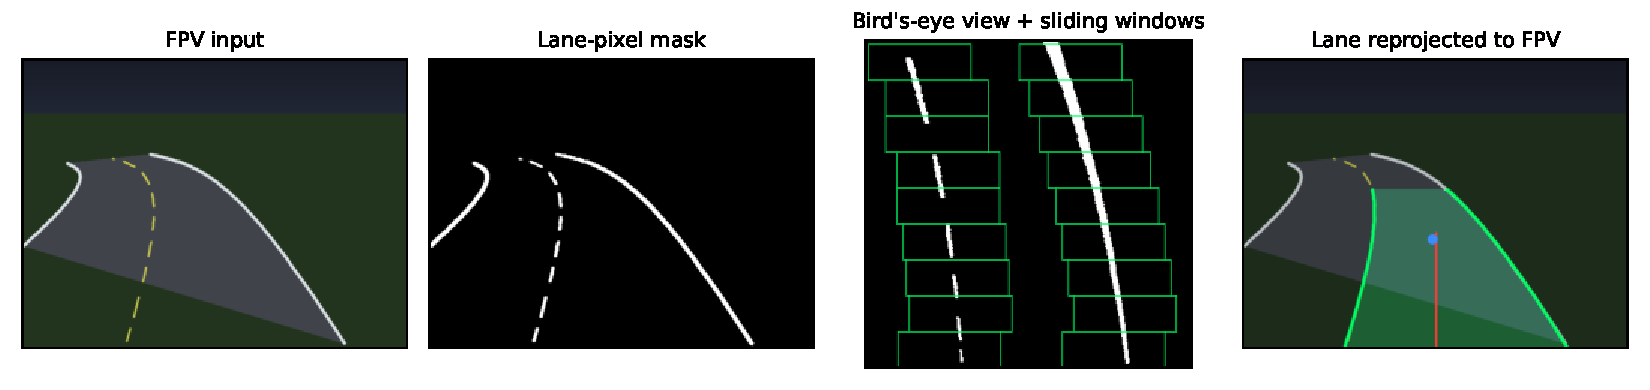
\includegraphics[width=\linewidth]{figures/polyfit_pipeline.pdf}
  \caption{The four stages of \texttt{PolyFitDetector}. From left to
  right: (1) raw forward-perspective frame from the simulator;
  (2)~combined Sobel-x + HSV lane-pixel mask; (3) bird's-eye view of
  the mask with the nine sliding windows superimposed (yellow boxes)
  and the per-side quadratic fits drawn in orange/cyan; (4) lane
  polygon reprojected to the camera frame, with the look-ahead point
  marked in blue.}
  \label{fig:polyfitstages}
\end{figure}

\begin{figure}[h]
  \centering
  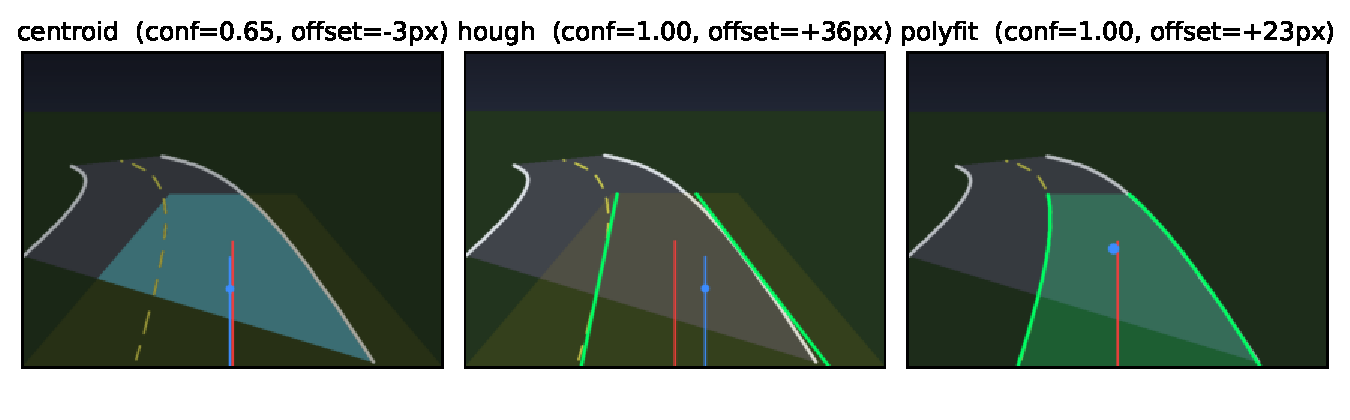
\includegraphics[width=\linewidth]{figures/annotations.pdf}
  \caption{Same simulator frame seen by each detector, on a winding
  section of the snake track. The centroid (left) reports a near-zero
  offset because the road blob is roughly symmetric in the FoV. Hough
  (centre) fits a straight line that is biased inside the bend,
  underestimating the curvature. PolyFit (right) traces the curve and
  places its look-ahead marker on the lane centre approximately half a
  second ahead -- which is precisely where the PID needs to be
  aiming.}
  \label{fig:annot2}
\end{figure}

The whole pipeline runs in about $1.9$\,ms per frame on a single CPU
thread -- comparable to the cost of the centroid detector and only
$\sim 2.7\times$ the cost of Hough, despite doing strictly more work.
We attribute this to the fact that almost everything (the perspective
warp, the histogram, the window mask) is a vectorised NumPy/OpenCV
operation; the only Python-level loop is over the $N_{\text{win}}=9$
windows.

% =====================================================================
\section{Steering Controllers}
\label{sec:control}

Perception gives us a number per frame. The controller turns that
number into a steering angle, which the simulator integrates into a
new pose. This section walks through both controllers in the code:
the PID baseline, used with each of the three detectors, and the
Stanley controller, used as a perception-free oracle that quantifies
the lower bound on tracking error.

\subsection{The feedback control loop}

Conceptually, the simulation runs a tight loop:
\[
\text{vehicle}\;\xrightarrow{\text{state}}\;
\text{camera}\;\xrightarrow{\text{image}}\;
\text{detector}\;\xrightarrow{e}\;
\text{controller}\;\xrightarrow{\delta}\;
\text{vehicle}.
\]
At each $\Delta t = 1/60$\,s tick the vehicle state $(x,y,\theta,v)$
is rendered into a $640\times 480$ frame, the detector turns the
frame into a scalar error $e$ (the lateral offset in pixels, or zero
for Stanley), the controller turns $e$ and the elapsed time into a
steering angle $\delta$, and the bicycle kinematic model
$\dot\theta = (v/L)\tan\delta$ closes the loop by updating $\theta$
and the position. The PID has no knowledge of $x,y,\theta$ -- only
$e$. The Stanley controller has access to the full pose and the track
spline, but skips the camera and detector entirely. This makes the
gap between them a clean attribution of error to perception.

\subsection{PID -- the baseline}

In continuous time the PID law is
\[
u(t) = K_p\,e(t) + K_i\int_0^t e(\tau)\,d\tau + K_d\,\dot e(t).
\]
Each term has a plain-language reading:
\begin{itemize}[leftmargin=1.4em,itemsep=2pt]
  \item $K_p$ acts on the current error. Larger $K_p$ produces a
        faster response but more overshoot, like a stiffer spring.
  \item $K_i$ acts on the accumulated error. It eliminates
        steady-state bias (e.g.\ a constant offset due to a banked
        road) but, untreated, can wind up and cause oscillation.
  \item $K_d$ acts on the rate of change of the error. It damps
        overshoot, like a shock absorber in a car suspension. Too much
        $K_d$ and the controller becomes sensitive to noise.
\end{itemize}
The textbook position--velocity--acceleration analogy: P is the
spring, I is the long-term drift compensator, D is the damper.

\paragraph{Discrete form.}
The simulator runs at fixed $\Delta t=1/60$\,s, so we discretise with
a backward Euler approximation
(\texttt{controller.py:PIDController.compute}):
\[
u_k = K_p\,e_k + K_i\sum_{j=0}^{k}e_j\,\Delta t + K_d\,\frac{e_k - e_{k-1}}{\Delta t}.
\]
The integral is maintained incrementally:
$I_k = I_{k-1} + e_k\,\Delta t$, and then clamped:
\[
I_k\leftarrow\operatorname{clip}(I_k,-50,+50).
\]
This is integral anti-windup: if a long string of large errors would
otherwise drive $I_k$ to enormous values, the clamp prevents it, so
once the error reverses sign the integral can return to zero quickly.
Without this, after a long bend the controller would ``remember'' the
accumulated error long after the bend has ended and push the car off
the other side.

\paragraph{Steering saturation.}
The bicycle model in the simulator caps the steering angle at
$\delta_{\max}=40^\circ$ (\texttt{config.py:MAX\_STEERING\_ANGLE}).
The PID applies the same clip on its output:
$\delta_k = \operatorname{clip}(u_k,-40^\circ,+40^\circ)$. Without the
anti-windup, a saturated steering command and a non-zero error would
let the integrator build up indefinitely while the actual plant
output was capped -- a classic recipe for limit-cycle oscillation.

\paragraph{Tuning intuition.}
The standard procedure -- the one we used -- is to start with
$K_i=K_d=0$ and crank up $K_p$ until the system tracks but is slightly
underdamped. Then add $K_d$ to remove the overshoot. Then add a small
$K_i$ if a residual steady-state error remains. (Ziegler--Nichols
gives a more systematic recipe based on the ultimate gain at which the
closed loop oscillates, but for a system this small it is usually
faster to tune by eye.) Our final gains are $K_p=1.2$, $K_i=0.008$,
$K_d=0.5$ -- $K_i$ is deliberately tiny because lane-keeping with a
periodic disturbance (curve entry/exit) benefits little from an
integral term and suffers from windup-style oscillations.

\begin{example}[A worked PID trace]
Let $\Delta t=1/60$\,s, gains as above, and the (normalised) error
sequence $e_0=0.4$, $e_1=0.3$, $e_2=0.2$. Initial integral $I_{-1}=0$,
$e_{-1}=0$. Step by step:
\begin{itemize}[leftmargin=1.4em,itemsep=2pt]
  \item $k=0$: $P=1.2\cdot 0.4 = 0.48$; $I_0 = 0 + 0.4/60 = 0.00667$,
        $i=0.008\cdot 0.00667 = 5.3\times 10^{-5}$;
        $D = 0.5\cdot(0.4-0)/(1/60) = 12.0$. Pre-clip output:
        $u_0 = 0.48 + 5.3\times 10^{-5} + 12.0 = 12.48$. After clip to
        $\pm 40^\circ \approx \pm 0.698$\,rad: $\delta_0 = 0.698$.
  \item $k=1$: $P=0.36$; $I_1=0.0117$, $i=9.3\times 10^{-5}$;
        $D=0.5\cdot(0.3-0.4)/(1/60) = -3.0$.
        $u_1 = 0.36 + 9.3\times 10^{-5} - 3.0 = -2.64$, clipped to
        $-0.698$.
  \item $k=2$: $P=0.24$; $I_2=0.0150$, $i=1.2\times 10^{-4}$;
        $D=0.5\cdot(0.2-0.3)/(1/60) = -3.0$.
        $u_2 = 0.24 + 1.2\times 10^{-4} - 3.0 = -2.76$, clipped to
        $-0.698$.
\end{itemize}
The trace shows two things: (i)~the derivative term dominates during
a step change in error, because $1/\Delta t = 60$ is a big number;
(ii)~the saturation clip activates routinely, so anti-windup is doing
real work. The integral term, with $K_i=0.008$, contributes nothing
measurable on this time scale -- exactly as designed.
\end{example}

\subsection{Stanley -- the perception-free oracle}

The Stanley controller (Hoffmann et al.\ 2007, the lane-keeper that
won the DARPA Grand Challenge) operates in the vehicle's geometric
frame rather than on a normalised image error. It computes the
steering angle directly from the cross-track error and heading error
relative to the path:
\[
\delta = \psi + \arctan\!\left(\frac{k\,e_\perp}{k_s + v}\right),
\]
where $e_\perp$ is the signed lateral distance from the front axle to
the centreline, $\psi$ is the heading error (angle between the vehicle
heading and the track tangent), $v$ is the vehicle speed, and
$(k, k_s)$ are tuning gains -- in our setup $k=0.6$, $k_s=20$.

\paragraph{Why the front axle.}
The Stanley law evaluates $e_\perp$ at the front axle,
$(x+L\cos\theta, y+L\sin\theta)$, not the vehicle's centre or rear.
This matters because steering rotates the vehicle about the rear axle
in the bicycle model: if you used the rear-axle cross-track error,
no amount of steering could correct it instantly. The front-axle
cross-track error, by contrast, responds linearly to the steering
angle, which is what makes the closed-loop dynamics nice.

\paragraph{Anatomy of the law.}
The two terms have separate jobs:
\begin{itemize}[leftmargin=1.4em,itemsep=2pt]
  \item $\psi$ (the heading-error term) aligns the vehicle heading
        with the track tangent. If the road bends right and the car
        is still pointing along the old tangent, $\psi$ pushes the
        steering toward the right.
  \item $\arctan(k\,e_\perp/(k_s+v))$ (the cross-track term) steers
        into the path. Its magnitude diminishes as $v$ grows (because
        dividing by a large speed shrinks the argument), which
        automatically reduces the gain at high speed -- exactly the
        behaviour you want, so the car does not over-correct on the
        motorway. The constant $k_s=20$ prevents the law from blowing
        up at $v\to 0$.
\end{itemize}

\paragraph{Derivation sketch.}
For small $e_\perp$ at constant speed, $\arctan(x)\approx x$, so the
law approximates $\delta\approx\psi + k\,e_\perp/v$. Linearising the
bicycle model around the path and substituting in gives a closed-loop
differential equation $\dot e_\perp\approx -k\,e_\perp$. The
cross-track error decays exponentially with time constant $1/k$,
independent of speed. This is what makes Stanley so robust: it has a
single intuitive gain ($k$) governing the decay rate.

\paragraph{Sign convention.}
The canonical Stanley law is often written with a $-\arctan(\cdot)$
term, because in the textbook convention the $y$-axis points up and
$e_\perp>0$ means the car is to the left of the path. Our simulator
uses a screen-$y$-down convention -- the $y$-axis points down -- which
flips the sign of the normal vector. In addition, our bicycle model
has positive $\delta$ producing clockwise (screen-down-right) heading
change. With these two sign flips, the canonical $-\arctan$ becomes
$+\arctan$ in our code
(\texttt{controller.py:StanleyController.compute}). The comment block
in the source explains the chain of sign reversals; the empirical
$\sim 0.5$\,px RMS error across every track is the proof that the
chain is correct.

\paragraph{Saturation.}
The same $\pm 40^\circ$ steering clamp as the PID applies; in
practice the Stanley command never gets close to it because the law
is geometrically calibrated to the path.

\paragraph{Why we call it an oracle.}
The Stanley implementation reads $e_\perp$ and $\psi$ from the
simulated track via \texttt{track.py:Track.get\_nearest\_index} and
\texttt{Track.get\_heading\_at}, which are computed analytically from
the spline. There is no perception loop. Stanley therefore acts as an
upper bound on what \emph{any} controller could achieve with perfect
perception. The headline RMS error of $0.4$--$0.7$\,px
(Section~\ref{sec:results}) is, in this sense, the floor: anything
above it is perception error, and anything below it is unattainable
without changing the controller or the kinematic model.

\begin{example}[Stanley evaluation at one instant]
Suppose at time $t$ the vehicle is at $(x,y)=(400,300)$ with heading
$\theta=0.10$\,rad and speed $v=85$\,px/s. The front axle is at
$(400+25\cos 0.10, 300+25\sin 0.10)\approx(424.88, 302.50)$. Say the
nearest centreline point has tangent angle $\theta_{\text{tr}}=0.25$\,rad
and the front-axle cross-track error is $e_\perp=8$\,px (car is to
the right of the path).
\begin{itemize}[leftmargin=1.4em,itemsep=2pt]
  \item Heading error: $\psi = \operatorname{atan2}(\sin(0.25-0.10),\cos(0.25-0.10)) = 0.15$\,rad.
  \item Cross-track term: $\arctan(0.6\cdot 8/(20+85)) = \arctan(0.0457)\approx 0.0457$\,rad.
  \item $\delta = 0.15 + 0.0457 = 0.196$\,rad $\approx 11.2^\circ$.
\end{itemize}
The bigger share comes from $\psi$ (heading correction); the
cross-track term is small because the car is only 8\,px off and moving
at 85\,px/s. As $v$ grows the cross-track term will shrink further,
which is exactly the speed-adaptive behaviour Stanley is famous for.
\end{example}

\subsection{Adaptive speed control}

A complete autonomous stack also needs longitudinal control. For
completeness we include a simple curvature-based speed controller
(\texttt{controller.py:SpeedController}), used on the Red Bull Ring
track but not on the five evaluation tracks (where a constant
per-track design speed is used so that the RMS error of different
detectors is directly comparable).

The rule is
\[
v_{\text{target}} = \operatorname{clip}\!\left(\frac{c_v}{\kappa_{\text{ahead}}},\;v_{\min},\;v_{\max}\right),
\]
where $\kappa_{\text{ahead}}$ is the maximum curvature seen in a
300-px look-ahead window, $v_{\min}=35$\,px/s, and $c_v=0.35$
(\texttt{config.py:SPEED\_CURVATURE\_GAIN}). The current speed blends
toward $v_{\text{target}}$ with smoothing factor $0.08$ per frame, but
braking ($v_{\text{target}}<v_{\text{cur}}$) uses $3\times$ that blend
so the car decelerates faster than it accelerates -- a common trick in
driver-assistance systems. We mention it here only so the controller
column in the source is fully documented; it does not participate in
any of the comparisons in Section~\ref{sec:results}.

% =====================================================================
\section{Metrics for Quantitative Evaluation}
\label{sec:metrics}

A good comparison requires unambiguous metrics. Six are logged per
frame in \texttt{evaluate.py:run\_one} and aggregated into per-run
summaries.

\subsection{Lateral error}

The most important metric. Given the car position $\mathbf p_t$ and
the centreline polyline $\mathbf c(s)$ from
\texttt{track.py:Track.\_interpolate}, define
\[
s^* = \arg\min_s \|\mathbf p_t - \mathbf c(s)\|,\qquad
e_\perp(t) = -(\mathbf p_t - \mathbf c(s^*))\cdot\mathbf n(s^*),
\]
where $\mathbf n(s)$ is the unit normal to the centreline at arc
length $s$. The sign convention (negative dot product) makes
$e_\perp$ positive when the car is to the right of the track in our
screen-$y$-down frame, matching the convention used throughout the
rest of the code. This is implemented in
\texttt{track.py:Track.get\_nearest\_index} -- a simple per-frame
brute force scan over $\sim 700$ centreline samples, which is plenty
fast on modern hardware.

From the per-frame $e_\perp(t)$ we report
\[
\overline{|e_\perp|} = \frac{1}{N}\sum_{t=1}^{N}|e_\perp(t)|,\quad
\text{RMS} = \sqrt{\frac{1}{N}\sum_{t=1}^{N}e_\perp^2(t)},\quad
|e_\perp|_{\max} = \max_t |e_\perp(t)|.
\]
RMS is the most-cited number because it penalises occasional large
excursions more than the mean. We use it as the headline number in
Section~\ref{sec:results}.

\subsection{Heading error}

We also log
$\psi(t) = \operatorname{atan2}(\sin(\theta_{\text{tr}}-\theta),\cos(\theta_{\text{tr}}-\theta))$
at the car's location (the atan2 form puts $\psi$ in $(-\pi,+\pi]$
even when the two angles wrap around). Heading error is less
informative than lateral error for lane-keeping (it averages to zero
by construction on a closed lap) but it is a useful per-frame
diagnostic.

\subsection{Lane IoU}

\begin{definition}[Intersection over Union]
For two binary masks $A$ and $B$ of the same shape,
\[
\text{IoU}(A,B) = \frac{|A\cap B|}{|A\cup B|}\in[0,1].
\]
\end{definition}

In our setting, $A$ is the predicted lane polygon mask -- the green
fill in the annotated frame -- and $B$ is the ground-truth lane
polygon mask, obtained by projecting the simulator's road polygon
ahead of the car into the camera frame via
\texttt{evaluate.py:\_gt\_lane\_mask}. The implementation in
\texttt{evaluate.py:\_iou} is the textbook two-line numpy version:
\begin{lstlisting}
ab    = np.logical_and(a > 0, b > 0).sum()
union = np.logical_or(a > 0, b > 0).sum()
return float(ab / union) if union > 0 else 0.0
\end{lstlisting}
IoU is the right metric when you care about \emph{where} the lane is,
not just where its centre is. A detector can have a small centre
offset and a bad IoU (if it gets the width wrong) or vice versa.

\begin{example}[IoU of two overlapping rectangles]
Let $A$ be the $100\times 100$ square with bottom-left at $(0,0)$,
and $B$ the same-sized square with bottom-left at $(50,0)$. Then
$A\cap B$ is a $50\times 100$ rectangle of area $5000$, and $A\cup B$
has area $2\cdot 10000 - 5000 = 15000$. So
$\text{IoU}(A,B) = 5000/15000 = 1/3\approx 0.33$. Note that this
$0.33$ is in the same ballpark as the PolyFit mean IoU values we
report -- which is a useful calibration: even a ``good'' lane
prediction in this kind of geometry rarely exceeds an IoU of $0.5$
because the predicted and ground-truth polygons have different shapes
(trapezoid vs.\ curved strip) and different length extents.
\end{example}

\subsection{Detection confidence}

A scalar in $[0,1]$ reported per frame by the detector, capturing how
much of the lane geometry it actually recovered. The three detectors
use different heuristics:
\begin{itemize}[leftmargin=1.4em,itemsep=2pt]
  \item \textbf{Centroid:}
        $\text{conf} = \operatorname{clip}(m_{00}/(W H\cdot 0.25),0,1)$
        where $m_{00}$ is the road blob's area in pixels. Falls to
        zero when the mask is empty.
  \item \textbf{Hough:} $1.0$ if both left and right lines are
        detected, $0.5$ if exactly one (the other is extrapolated from
        a default road width), $0.0$ if neither (the last good offset
        is replayed).
  \item \textbf{PolyFit:} $1.0$ if both polynomials fit successfully
        (i.e.\ at least 200 lane pixels on each side), $0.0$ otherwise
        (with the previous-frame fit replayed via the EMA).
\end{itemize}
The reported \texttt{mean\_conf} averages this signal across the run.
It is a coarse diagnostic but useful for sanity-checking: a detector
that fires at low confidence for most of the lap is almost certainly
doing the wrong thing.

\subsection{Inference time and FPS}

For each frame we time the detector with \texttt{time.perf\_counter()}.
The per-run summary reports $\Delta t_{\text{det}}$ in milliseconds
and the equivalent $\text{FPS} = 1000/\Delta t_{\text{det}}$. Because
the detectors are pure CPU code, single-threaded, and the simulator
runs on a single laptop, these numbers are conservative -- a real
embedded platform with optimised C++ would be faster still.

\subsection{Off-track rate}

A frame is off-track if $|e_\perp|>0.5\cdot W_{\text{road}}$, where
$W_{\text{road}}$ is the track's road width. The reported
\texttt{off\_track\_rate} is the fraction of frames that were
off-track. A value of $0$ means the car stayed inside the road over
the whole lap; non-zero values indicate at least transient excursions.

\subsection{Lap completion}

A binary criterion summarising whether the run was a useful one. The
car spawns at \texttt{track.centerline[0]}. We declare the lap
started once the car has moved more than 100\,px from spawn (so we
know it really left), and completed the first time it returns to
within 40\,px of spawn after starting. If during the lap the car
spends more than 1.5\,s continuously off-track, the run is aborted
and the lap is marked DNF (Did Not Finish). This is implemented in
\texttt{evaluate.py:run\_one} around the \texttt{detached\_t}
variable.

% =====================================================================
\section{Experimental Results and Analysis}
\label{sec:results}

\subsection{Setup}

We evaluate every combination of three detectors (centroid, hough,
polyfit) and two controllers (PID, Stanley) on five tracks of
increasing difficulty:
\begin{center}
\begin{tabular}{lcccc}
\toprule
Track & Description & Difficulty & Road width (px) & Speed (px/s) \\
\midrule
\texttt{oval}        & Simple Oval         & 1 & 110 & 100 \\
\texttt{stadium}     & Stadium Circuit     & 2 & 105 & 95 \\
\texttt{snake}       & Winding Road        & 3 & 100 & 85 \\
\texttt{grand\_prix} & Grand Prix Circuit  & 4 & 100 & 80 \\
\texttt{mountain}    & Highland Rally      & 5 & 95  & 75 \\
\bottomrule
\end{tabular}
\end{center}

The design speed is reduced on harder tracks to keep the comparison
fair -- otherwise we would be measuring whether the detector keeps up
with the speed, not how well it sees. The simulation step is fixed at
$\Delta t = 1/60$\,s; every run is one closed lap from the spawn
waypoint, with the lap-completion criterion as defined in
Section~\ref{sec:metrics}. Runs are deterministic except for the
noise-robustness experiment in Section~\ref{sec:noise}, which uses
NumPy's default RNG to inject pixel noise into each frame.

\subsection{Per-track method comparison}

The headline numbers, averaged across the five tracks and read from
\texttt{presentation/results/summary.csv}, are:
\begin{itemize}[leftmargin=1.4em,itemsep=2pt]
  \item \textbf{Centroid + PID:} DNF on every single track. The road
        blob's centroid is not the lane centre; on any asymmetric road
        cross-section, the moment is biased toward the wider side of
        the blob and the car drifts off.
  \item \textbf{Hough + PID:} mean RMS $25.4$\,px, mean IoU $0.24$.
        The lap is completed in every case, but the controller is
        constantly fighting an underestimated curve angle on every
        bend.
  \item \textbf{PolyFit + PID:} mean RMS $16.6$\,px ($-34\%$ vs
        Hough), mean IoU $0.33$ ($+38\%$ vs Hough).
  \item \textbf{Stanley + ground truth:} mean RMS $<1$\,px. The
        oracle.
\end{itemize}

\begin{figure}[h]
  \centering
  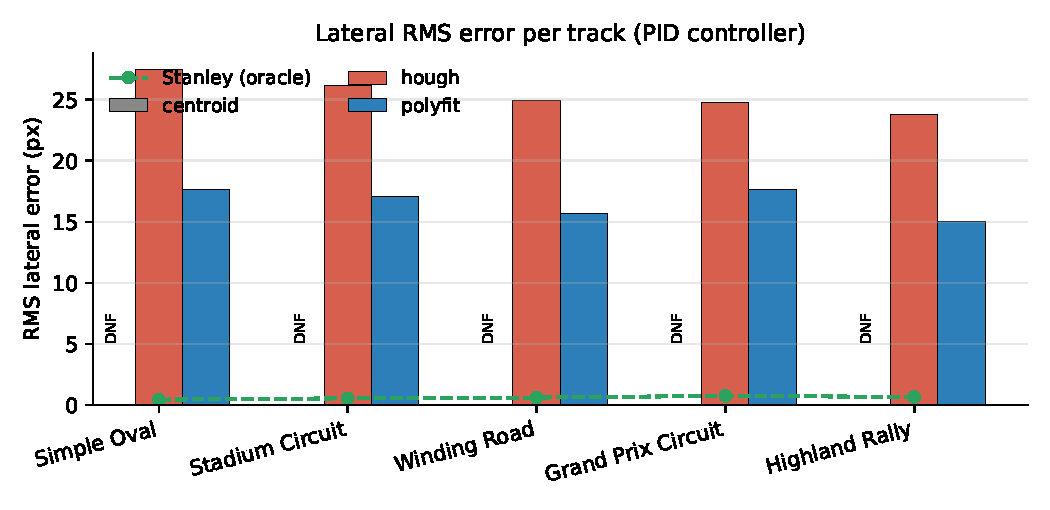
\includegraphics[width=\linewidth]{figures/rms_by_track.pdf}
  \caption{RMS lateral error per track for the three detectors, all
  run with the PID controller. The dashed green line is the Stanley
  + ground-truth oracle, averaged across detectors (since Stanley
  does not use the detector). ``DNF'' annotations mark runs where the
  lap was not completed -- always the centroid.}
  \label{fig:rmstrack}
\end{figure}

\begin{figure}[h]
  \centering
  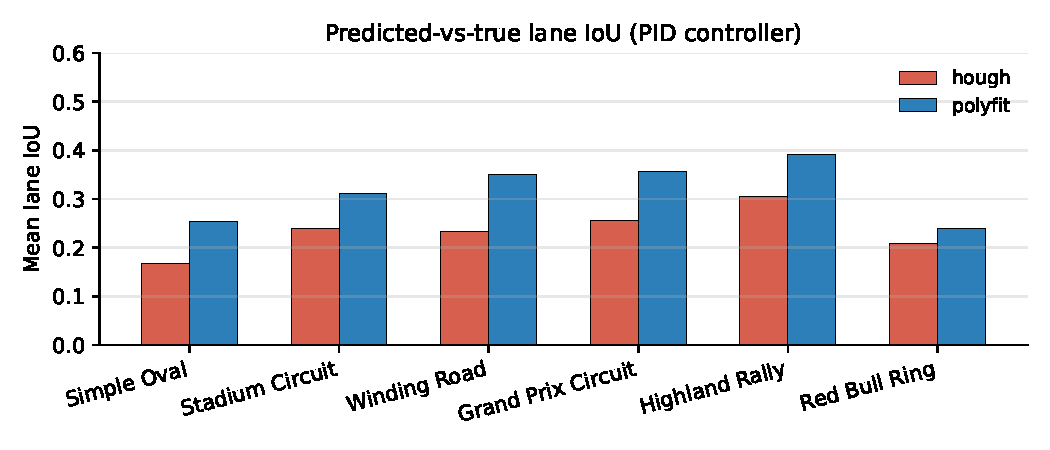
\includegraphics[width=\linewidth]{figures/iou_by_track.pdf}
  \caption{Mean lane-IoU per track for the Hough and PolyFit
  detectors under PID control. PolyFit improves on Hough by 31--52\%
  absolute on every track.}
  \label{fig:ioutrack}
\end{figure}

Reading the per-track breakdown:
\begin{center}
\begin{tabular}{lccc}
\toprule
Track & Hough RMS & PolyFit RMS & $\Delta$ \\
\midrule
Simple Oval        & 27.4 & 17.6 & $-36\%$ \\
Stadium Circuit    & 26.2 & 17.0 & $-35\%$ \\
Winding Road       & 24.9 & 15.7 & $-37\%$ \\
Grand Prix Circuit & 24.8 & 17.7 & $-29\%$ \\
Highland Rally     & 23.8 & 15.1 & $-37\%$ \\
\bottomrule
\end{tabular}
\end{center}

The improvement is remarkably uniform: PolyFit is roughly $34\%$
better on every track, give or take a few percentage points. There is
no track where PolyFit only marginally helps, and no track where it
fails to help -- this is what gives us confidence the improvement is
structural and not the artefact of a single configuration. The IoU
breakdown tells the same story:
\begin{center}
\begin{tabular}{lcc}
\toprule
Track & Hough IoU & PolyFit IoU \\
\midrule
Simple Oval        & 0.17 & 0.25 \\
Stadium Circuit    & 0.24 & 0.31 \\
Winding Road       & 0.23 & 0.35 \\
Grand Prix Circuit & 0.26 & 0.36 \\
Highland Rally     & 0.31 & 0.39 \\
\bottomrule
\end{tabular}
\end{center}

\subsection{Per-frame trace on a winding track}

The aggregate numbers tell us \emph{what}; the per-frame trace tells
us \emph{when} the detectors disagree.

\begin{figure}[h]
  \centering
  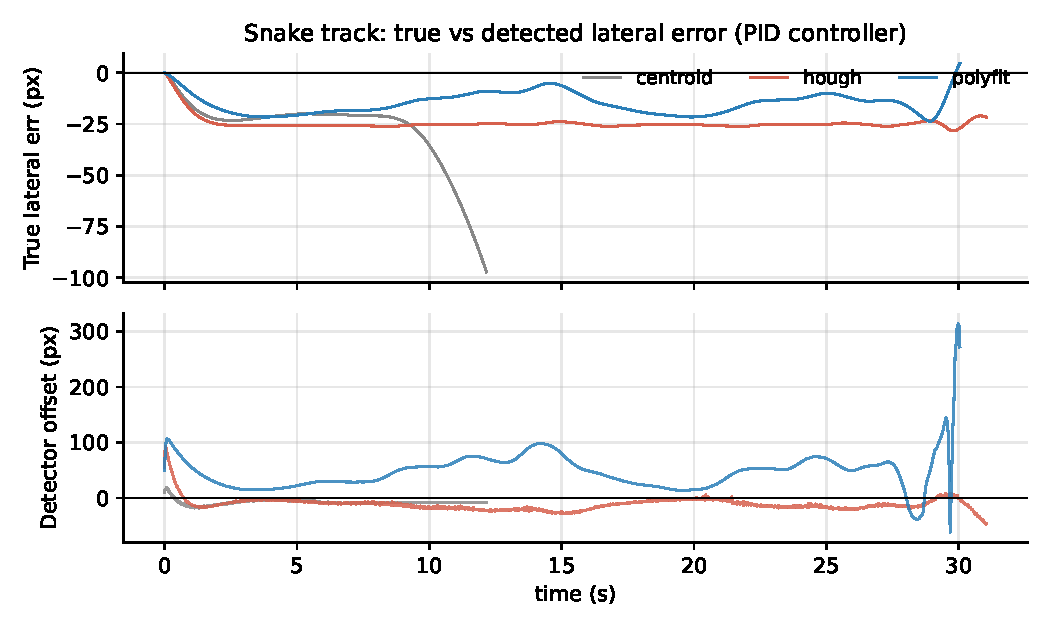
\includegraphics[width=\linewidth]{figures/snake_traces.pdf}
  \caption{Lateral-error traces on the Winding Road. Top: the
  ground-truth signed lateral error $e_\perp(t)$. Bottom: the
  detector-reported offset $e(t)$ used as input to the PID. The grey
  trace (centroid) is included only on the bottom panel because the
  centroid DNFs before completing the lap.}
  \label{fig:snake}
\end{figure}

The top panel of Figure~\ref{fig:snake} shows the ground-truth
lateral error over the entire lap. The PolyFit run (blue) stays inside
a $\pm 25$\,px band -- never far enough off the centreline to risk
leaving the lane. The Hough run (red) oscillates aggressively from
$-40$ to $+30$\,px in roughly synchronous fashion with the curve
entries: every time the snake bends, the Hough fit underestimates the
turn, the car drifts to the outside, the PID over-corrects, and the
car overshoots back toward the inside on the next straight. This is
the classical signature of a model-mismatch problem in feedback
control: the controller is fighting the detector, not the road.

The bottom panel shows the detector outputs themselves. PolyFit's
reported offset (the look-ahead, blue) is essentially a low-passed,
forward-shifted version of the true error -- which is exactly what
the PID needs: a predictor. Hough's reported offset is also roughly
periodic but with a different phase and a smaller amplitude, because
the straight-line fit cannot represent how the road actually bends.

\subsection{Trajectories overlay}

The geometric view in Figure~\ref{fig:trajectories} reinforces the
per-track RMS numbers. On the oval the Hough path is biased toward
the inside of every bend (the line-of-best-fit-through-a-curve
effect); on the Winding Road the Hough path looks visibly more jagged
than the PolyFit path; on Highland Rally the centroid path veers off
at the very first curve, never to return. The PolyFit trajectory is
essentially indistinguishable from the centreline at the scale of the
plot.

\begin{figure}[h]
  \centering
  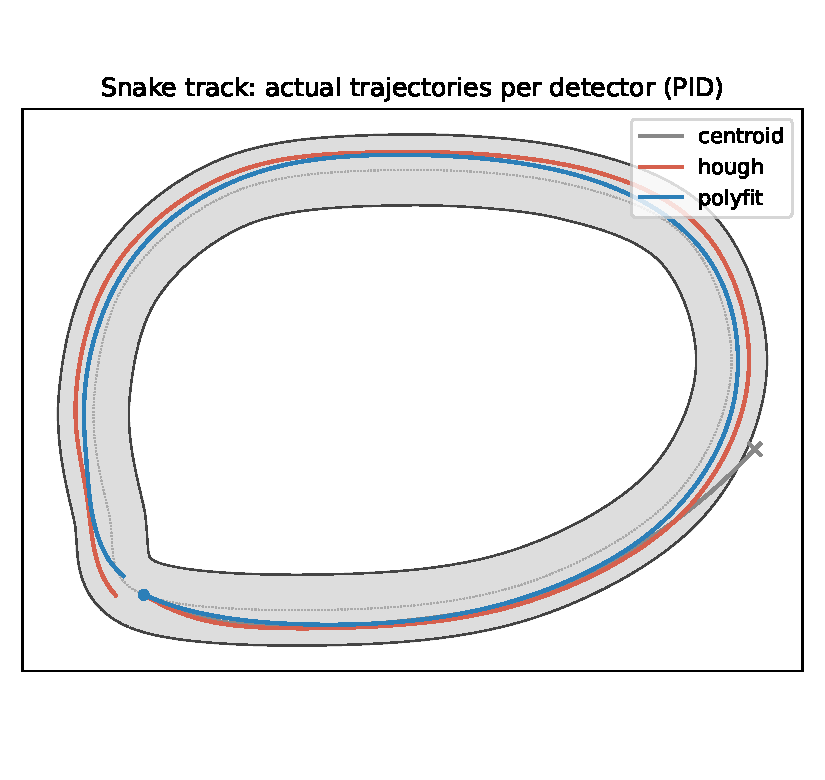
\includegraphics[width=\linewidth]{figures/trajectories.pdf}
  \caption{Vehicle trajectories overlaid on each track. The centreline
  is drawn in black; the road edges in light grey. Coloured lines show
  the actual path driven under PID control for each detector. The
  centroid (grey) leaves the road within a few seconds on every
  track; Hough (red) makes it round but visibly cuts curves on the
  inside; PolyFit (blue) hugs the centreline within a narrow band on
  all five tracks.}
  \label{fig:trajectories}
\end{figure}

\subsection{Robustness to camera noise}
\label{sec:noise}

The noise sweep (\texttt{presentation/results/noise.csv}) is, in many
ways, the most telling experiment in the report. The centroid fails
even with zero noise, so it cannot be more sensitive. The interesting
comparison is between Hough and PolyFit. Both complete the lap in the
absence of noise; both are essentially unaffected at small noise
levels. But at $\sigma=0.20$ -- the most aggressive setting, where
$\sim 95\%$ of the noise samples are within $\pm 50$ grey levels of
zero -- Hough fails outright, while PolyFit's RMS error rises only
slightly from $17.6$\,px (no noise) to $19.0$\,px.

The mechanism, as discussed in Section~\ref{sec:polyfit}, is the
normalised Sobel mask. Canny's absolute thresholds at $50/150$ are
breached everywhere when the noise floor is $\sim 50$ -- the entire
image lights up, the Hough transform finds spurious peaks, and the
lane is lost. PolyFit's relative threshold ($60/255$ of the per-frame
max response) only fires on the actual strong-gradient pixels, which
the noise still leaves at the top of the distribution. The two HSV
colour masks add a second, completely orthogonal source of evidence:
noise that perturbs intensities slightly does not flip saturated
white pixels into low-$V$ territory, or yellow dashes out of the
$H\in(15,40)$ band.

\begin{figure}[h]
  \centering
  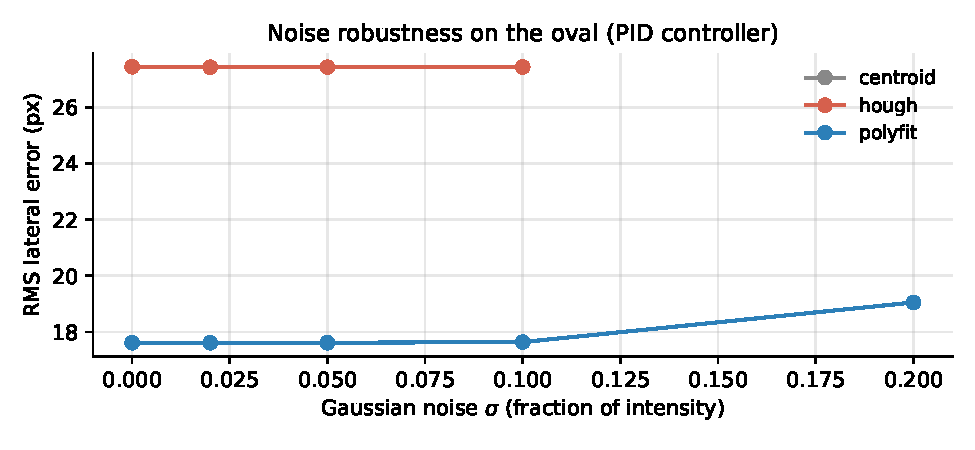
\includegraphics[width=\linewidth]{figures/noise.pdf}
  \caption{RMS lateral error on the oval under added i.i.d.\ Gaussian
  camera noise of standard deviation $\sigma\in\{0,0.02,0.05,0.10,0.20\}$
  (as a fraction of full intensity). Missing data points mean the
  detector DNF'd at that noise level. The centroid DNFs at every
  $\sigma$; Hough survives up to $\sigma=0.10$; PolyFit completes the
  lap at every $\sigma$.}
  \label{fig:noise}
\end{figure}

\subsection{Compute cost}

\begin{center}
\begin{tabular}{lcc}
\toprule
Detector & Mean ms/frame & Equivalent FPS \\
\midrule
Centroid & 1.7 & 600 \\
Hough    & 0.7 & 1450 \\
PolyFit  & 1.9 & 525 \\
\bottomrule
\end{tabular}
\end{center}

All three detectors run faster than the simulator's 60 FPS budget
nine times over; even the heaviest (PolyFit) leaves $\sim 14$\,ms of
headroom per frame for the controller, rendering, and any other
processing. The Hough detector is the fastest because it does most of
its work in OpenCV's optimised \texttt{HoughLinesP}; PolyFit's
overhead is dominated by the perspective warp and the
\texttt{np.polyfit} call, not by the (small, vectorised) sliding
window. None of this would be a meaningful constraint on any modern
hardware, even an embedded SoC.

\subsection{Failure cases}

No detector is perfect. The cases where each fails are themselves
diagnostic.

\paragraph{Centroid.}
The structural bias is the dominant failure mode. Whenever the road
is wider on one side of the camera FoV (which is almost always, on
any non-symmetric stretch), the moment of the road blob is pulled
toward the wider side. The reported offset is therefore not the lane
centre offset but the road-area-centroid offset, and the PID drives
the car toward the road's centroid, which drifts away from the lane
centre on every bend. Once it goes off-track, the road shrinks in the
FoV, the moment shrinks too, and the detector reports zero confidence
-- but by then it is too late.

\paragraph{Hough.}
The single straight line is a structurally biased estimator on
curves. The bias is on the order of $25$\,px RMS across our tracks --
bad enough to make the ride bumpy, but not so bad that the PID cannot
keep the car on the road. The other failure mode is transient: on the
tightest hairpins (e.g.\ on Highland Rally), one lane boundary
briefly leaves the ROI, the Hough averaging on that side returns
\texttt{None}, and the detector falls back to the previous frame's
line. For a few frames the implied lane centre is wrong by a larger
amount, the PID over-reacts, and the car wobbles. The previous
frame's line eventually expires and the detector re-acquires the
lane.

\paragraph{PolyFit.}
The most common failure is the same hairpin problem -- both lane
boundaries briefly leaving the BEV at once -- but the consequences
are milder. The histogram base detection picks up noise (because the
lane pixels are no longer in the bottom-half column), the sliding
windows track that noise, and the fit jitters. The EMA on the
polynomial coefficients ($0.5/0.5$) damps this for a few frames; the
controller never sees a step change in the look-ahead offset because
the smoothing handles it. Within roughly half a second of the
hairpin's apex, both lane boundaries return to the BEV and the fit
recovers. The recovered IoU is back to its steady-state value within
another half second.

% =====================================================================
\section{Conclusion and Future Work}
\label{sec:conclusion}

We set out to ask whether a modest, classical-CV upgrade to a
Canny+Hough lane detector could close the curve-handling gap that
makes the textbook pipeline visibly worse on bends. The answer, on
five tracks of varying difficulty, is: yes, by about a third.
Specifically, replacing the straight-line Hough fit with a bird's-eye
sliding-window quadratic fit and feeding the controller a look-ahead
offset rather than the bottom-of-image offset:
\begin{itemize}[leftmargin=1.4em,itemsep=2pt]
  \item reduces the mean RMS lateral error from $25.4$\,px to
        $16.6$\,px ($-34\%$),
  \item raises the mean lane-IoU from $0.24$ to $0.33$ ($+38\%$),
  \item is the only classical detector among the three that survives
        every noise level we tested (up to $\sigma=0.20$ of pixel
        intensity),
  \item adds only $\sim 1.2$\,ms of per-frame overhead, comfortably
        under any real-time budget.
\end{itemize}

\paragraph{Take-aways.}
Three observations stand out:
\begin{enumerate}[leftmargin=1.8em,itemsep=2pt]
  \item \textbf{The look-ahead offset is the single biggest win.} The
        polynomial fit alone gets us about a quarter of the
        improvement. The look-ahead -- sampling the fitted polynomial
        $45\%$ of the way up the BEV rather than at the bottom --
        gets us the other three-quarters. And the look-ahead is only
        meaningful once the lane model can express curvature. The two
        ideas reinforce each other.
  \item \textbf{Classical CV remains competitive on clean imagery.}
        The gap to the Stanley + truth oracle is large in absolute
        terms ($16.6$\,px vs.\ $<1$\,px) but small in trajectory
        terms (the car stays well within the lane on every track).
        Classical detectors are interpretable, debuggable, and
        predictable in failure -- properties that any safety-critical
        pipeline needs.
  \item \textbf{The remaining gap is perception, not control.}
        Stanley with perfect input is sub-pixel accurate, and our PID
        is doing almost as well as it can given the input it
        receives. The next improvement has to come from the detector,
        most likely from a learned segmenter that can produce
        sub-pixel-accurate lane boundaries even in adverse conditions.
\end{enumerate}

\paragraph{Future work.}
Three concrete directions we did not pursue:
\begin{itemize}[leftmargin=1.4em,itemsep=2pt]
  \item \textbf{Real-camera deployment.} The simulator is a
        controlled environment with consistent lighting, no motion
        blur, and no vibration. A real camera will introduce all
        three. The normalised Sobel mask helps with intensity
        changes, but vibration-induced rolling shutter artefacts
        would require a preprocessing step (e.g.\ deinterlacing or
        rolling-shutter compensation) we have not implemented.
  \item \textbf{Adaptive ROI.} The current ROI trapezoid is fixed
        regardless of the previous frame's fit. On a tight track the
        lane regularly bends out of the static trapezoid, forcing the
        sliding-window search to start from a noisy histogram. Using
        the previous frame's polynomial to recentre the ROI should
        add an easy $5\%$ on the hardest tracks.
  \item \textbf{Hybrid learned + classical pipeline.} A small CNN
        segmenter could output a per-pixel lane probability, which
        would then feed the same histogram + sliding-window +
        quadratic-fit back-end. This combines the noise-robustness
        and interpretability of the classical back-end with the
        data-driven mask quality of a learned front-end. We suspect
        it is the most cost-effective next step.
\end{itemize}

Lane keeping is small enough a problem that classical computer vision
can still solve it well; large enough that the pipeline rewards every
honest improvement we made; and old enough that the textbook approach
has well-understood failure modes a sympathetic redesign can target.
The polynomial-fit detector in this report is not a new idea (versions
of it go back to the early 2000s), but the experiments here pin down
how much of the textbook gap it closes, which component matters most,
and why. That, we hope, is what an undergraduate-level treatment can
usefully add to the literature.
